\section{Problema 2}

\subsection{Introducción}

En este problema se debe determinar el área total de un campo que queda protegida de una plaga de langostas. Para considerar aislada una porción del mismo, ésta debe estar completamente encerrada por vallas de altura mayor o igual a la del salto de las langostas. A partir de entender esto, pensamos de qué manera podíamos modelar el campo, partirlo en "porciones" (que luego llamaríamos \textit{parcelas}), y recorrerlas chequeando si podíamos infestarlas de langostas. Realizando este recorrido, esperábamos lograr identificar el área infestada y contando con el área total, obtener mediante una simple resta el área protegida.\\
\indent Debido a cómo está presentado el problema, y los datos de entrada, consideramos el campo como el primer cuadrante de un sistema de ejes cartesianos. Así, el molino donde se ubica la Tía queda representado por el origen - $(0,0)$ - y cada valla se ubica en el plano con respecto a este punto. Además, a partir de la longitud y orientiacón de cada valla inferimos el extremo donde termina. De esta manera, al procesarlas todas, pudimos obtener cuáles eran las coordenadas máximas en sentido del eje de ordenadas y abscisas, con lo cual fijamos los límites del campo sumando uno a esos valores.\\
\indent En un primer momento nos propusimos modelar el campo utilizando esta información pero volcándola en una matriz donde cada posición de la misma se correspondiera con un sector del campo de lado $1x1$. Nuestra idea era posicionar las vallas en la matriz, determinando qué cuadrados quedaban bloqueados, y luego infestar de alguna manera pintando las posiciones de la matriz a las que sí podíamos acceder. Rápidamente desistimos de esta idea (a pesar de que luego la retomaríamos optimizando nuestras estructuras) dado que manejarnos con esa matriz no nos permitía cumplir con la cota de complejidad pedida. Las dimensiones de la matriz hubieran sido proporcionales a la superficie del campo, la cual a su vez quedaba determinada por la ubicación de una valla, variable sobre la cual no podíamos suponer nada y no se relacionaba con las magnitudes que necesitábamos contar.\\
\indent El segundo intento consistió en pensar cada valla como un nodo de un grafo, donde las aristas estuvieran representadas por las intersecciones entre las vallas. Luego, los vecinos de un nodo/valla serían otros nodos/vallas con los que se tocara en cualquier punto. Viéndolo así, buscamos interpretar las porciones completamente valladas como los ciclos de ese grafo. Una vez que tuvieramos identificados los ciclos, debíamos ver cuáles eran válidos, cuáles incluían a otros, y así procesar demasiados casos particulares. No pudimos llegar a esa instancia, pues antes nos encontramos con la dificultad de contar e identificar ciclos. Sin embargo, al pensar en cómo podíamos clasificar los ciclos, introdujimos un detalle que luego perduraría en nuestra solución final: a medida que procesamos cada valla para alojarla en nuestra estructura dejamos de lado aquella cuya altura sea menor a la que saltan las langostas. Así nos aseguramos que en el resto del problema vamos a mirar vallas que sean candidatas a proteger una porción del campo, con lo cual prescindimos de realizar este chequeo y mirar vallas innecesariamente.\\
\indent Frente a un panorama incierto, y habiendo descartado dos intentos de solución, logramos desarrollar una tercera idea que terminaría siendo correcta para la resolución del problema tanto en términos de la solución esperada como de la complejidad temporal. 

\subsection{Representación del Problema}

El primer boceto de solución con que contamos intentaba trazar una cuadrícula sobre el campo y luego implementar eso sobre una matriz. Esto nos obligaba a movernos de a un paso a medida que infestabamos el terreno, transformando nuestra complejidad en algo que no se relacionaba con la cantidad de vallas, y que seguramente fuera muy superior a este número. Ahora bien, considerando este movimiento, concebimos que no tenía sentido pensar que la plaga de langostas se moviera en una dirección dada de a pasos tan pequeños ya que en última instancia podría moverse hasta que se topara con una valla, infestando en un solo paso grande varios de nuestros pequeños sectores anteriores.\\
\indent Dividimos entonces la representación del campo en distintas etapas de procesamiento (ver \textbf{Fig. ~\ref{fig:ej2Mapeo} }). Primero, extendimos las vallas iniciales en megavallas que atravesaran el terreno del campo de un extremo a otro. Para esto contamos con dos diccionarios de megavallas, uno correspondiente a las verticales y otro a las horizontales. Cada definición se hace en base a una clave (entero) que representa la coordenada vertical u horizontal en que se extiende esa megavalla, y un significado que no es otra cosa que una lista de las vallas originales que viven en ese segmento y cuya altura impide el salto de las langostas. Además, la manera en que representamos las vallas es a través de un par de coordenadas, cuyas componentes $x$ e $y$ indican el comienzo y fin de la valla respectivamente.

\clearpage

\begin{figure}[h]
\centering                                                       
        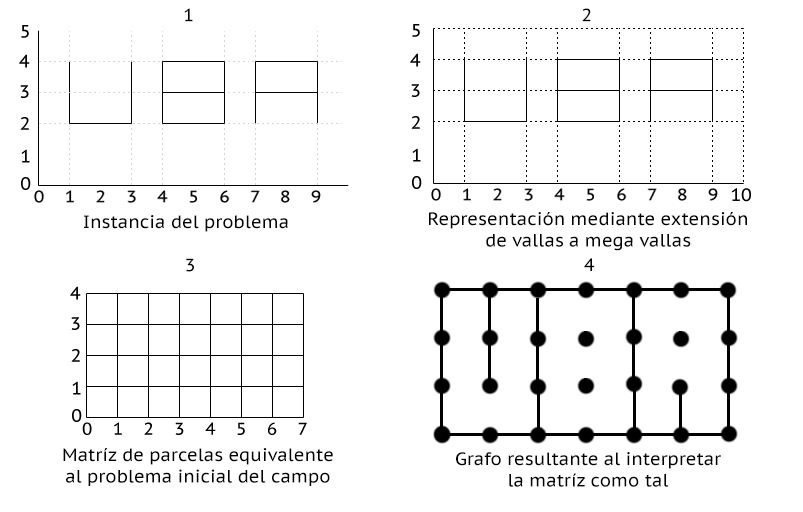
\includegraphics[width=320pt]{./figs/mapeoParcelas.png}
	\caption{Transformación del Problema Inicial}
	\label{fig:ej2Mapeo}
\end{figure}

Como se puede observar en la segunda imagen de la Fig. anterior, las intersecciones de las megavallas definen una cuadrícula de parcelas cuyo tamaño es variable y heterogéneo. Sin embargo, todas tienen forma rectangular, y a partir de la información almacenada hasta el momento es posible determinar su área y si el acceso a las parcelas contiguas está impedido o no por algún tramo de valla. Esto nos permitió armar una matriz que representara esta cuadrícula, de dimensiones $\#megavallasHor*\#megavallasVer$, y cuyas posiciones alojaran un objeto de tipo $Parcela$ que contuviera la información antes mencionada, además de agregar un atributo booleano para determinar si la parcela era infestable (necesario para recorrer la matriz con una adaptación de 'BFS'). Este procesamiento se realiza a través de la función $armarParcelas$ (ver \textsl{Pseudocódigo 2}). Para lograr el correcto armado y mapeo del campo a esta matriz necesitamos contar con las megavallas ordenadas en forma ascendente (garantizado por el diccionario) así como también las vallas contenidas en cada una. En un principio, implementamos cada megavalla como otro diccionario que tuviera como clave el comienzo de una valla y como significado su fin. Esto nos garantizaba el orden necesario para recorrerlas, pero nos imponía un costo logarítmico para acceder a su significado. Dado que esto nos arruinaba la complejidad, acudimos a la implementación de la colección de vallas mediante una lista de manera tal que, al terminar de procesar todas las vallas, ordenáramos cada colección y así pudieramos acceder a toda su información en tiempo constante. Por eso, en la resolución del problema, hay un llamado al método de Campo $ordenarVallas$ antes de armar la matriz de parcelas, pues en otro caso el algoritmo no sería correcto.\\
\indent Esta matriz de parcelas se corresponde con la etapa número 3 de la Figura ~\ref{fig:ej2Mapeo}. Como se explica en el análisis de complejidad, esta vez sí podemos pagar el costo de recorrer la matriz, ya que sus dimensiones se encuentran en función de la magnitud que nos interesa (\#vallas). Al interpretarla como un grafo, las posiciones (parcelas) pasaron a ser los nodos, mientras que la arista entre un par de nodos implica que las langostas pueden moverse de entre ambas parcelas contiguas (ver Fig. ~\ref{fig:ej2Mapeo}.4). Luego, todo el área que pudiera ser infestada por estos desalmados crustáceos representaría una componente conexa del grafo. Supusimos entonces que la plaga comenzaba a infestar el campo desde los bordes, con lo cual partiendo de la parcela origen aplicamos una adaptación de 'BFS' ($buscarArea$, \textsl{Pseudocódigo 3}) para infestar la componente conexa que contuviera los bordes. A través de este recorrido contamos el área que podía ser infestada, y luego se lo restamos al área total.

\clearpage


\subsection{Pseudocódigos}

\begin{algorithm}
\caption{armarParcelas (\textbf{in/out} campo: \textsl{Campo})}
\begin{algorithmic}[1]

\STATE $cantH \leftarrow$ cantidad de megavallas horizontales en el $campo$
\STATE $cantV \leftarrow$ cantidad de megavallas verticales en el $campo$
\STATE $cuadricula \leftarrow$ armar matriz de $cantH*cantV$
\WHILE{hay megavallas horizontales}
	\WHILE{hay megavallas verticales}
		\STATE crear una $parcela$ dada por las megavallas que la encierran
		\STATE definir en $parcela$ si se puede infestar en cada dirección
		\STATE definir en $parcela$ el área que comprende
		\STATE asignar $parcela$ a la posición correspondiente en $cuadricula$
	\ENDWHILE
\ENDWHILE
\STATE guardar $cuadricula$ en $campo$
\end{algorithmic}
\end{algorithm}

\begin{algorithm}
\caption{buscarArea (\textbf{in/out} campo: \textsl{Campo}) $\rightarrow$ res: \textsl{Integer}}
\begin{algorithmic}[1]

\STATE $cola \leftarrow$ crear cola de parcelas vacía
\STATE marcar $parcela$ $origen$ del campo como infestable
\STATE agregar $parcela$ $origen$ a la cola
\STATE $areaInfestada \leftarrow 0$

\WHILE{hay parcelas en la $cola$}
	\STATE $parcela \leftarrow$ pop primer elemento de la cola
	\STATE $areaInfestada \leftarrow areaInfestada$ $+$ área de $parcela$ 
	\STATE agregar parcelas contiguas a $parcela$ que se puedan infestar
\ENDWHILE
\RETURN área de $campo$ - $areaInfestada$
\end{algorithmic}
\end{algorithm}

\clearpage

\subsection{Demostración de Correctitud}

Para ver la correctitud del programa, es necesario analizar sus distintas etapas por separado y demostrar que cada una cumple con comportamiento descrito en el modelado del problema. La propuesta para esta demostración es comenzar desde el final y asumir que si valen ciertas condiciones sobre los parámetros de entrada, entonces el algoritmo $buscarArea$ resuelve el problema correctamente. Luego, basta con ir hacia atrás y probar que las distintas funciones que utilizamos para construir esos parámetros garantizan esas condiciones.\\

\textbf{Correctitud de \textit{buscarArea} }

\indent Para esta función contamos con un objeto de tipo $Campo$ que posee almacenada y procesada toda la información necesaria sobre la instancia del problema. En particular, nos interesa acceder a su matriz de parcelas y recorrerla tratando de infestar todo el terreno. Recordemos que cada parcela $p$ es rectangular y por lo tanto posee un entero indicando su área, una coordenada que hace referencia a su posición $(i,j)$ en la matriz, y cuatro booleanos que indican si por cada uno de sus cuatro lados se puede infestar la parcela contigua. Además, cuenta con un flag propio que indica si es infestable. Para el correcto funcionamiento de este algoritmo de búsqueda, todas las parcelas de la matriz deben tener este último booleano en $false$, pero sí deben contar con los indicadores correctos sobre si es posible infestar parcelas contiguas. Dado que esta función es una adaptación de 'BFS', a partir de una parcela dada irá agregarando a una cola aquellas parcelas contiguas que puedan ser infestadas y ya no hayan sido marcadas como tales (el equivalente a haber visitado un nodo).\\
\indent Debido a cómo fue construída, tanto la primera y última fila de la matriz como su primera y última columna corresponden a bordes del campo cuyas parcelas son infestables, pues asumimos que la plaga proviene desde cualquier dirección hacia el campo. Como esto impacta sobre el área total del campo, en principio el borde puede determinarse de manera arbitraria: lo importante es que exista, ya que sino el algoritmo no funcionaría como esperamos.\\
\indent Sea entonces $mp$ la matriz de parcelas de dimensiones $\#megaVallasH*\#megaVallasV$, este algoritmo comienza accediendo a la posición $(0,0)$ de la matriz para tomar la parcela $p_{0}$ y asignarle la condición de 'infestable'; luego la agrega a la cola y comienza el ciclo iterativo de recorrido. El invariante de nuestro algoritmo determina que cualquier parcela agregada a la cola puede ser infestada a través de alguna de sus parcelas vecinas (lo cual interpretamos como que exista una arista entre ambos nodos/parcelas), con lo cual esta suerte de 'BFS' se irá moviendo por la componente conexa que incluya a $p_{0}$ y a través de un efecto dominó infestará todas las parcelas en esta componente. Dado que garantizamos que hubiera al menos una fila o columna de parcelas borde infestables en cada extremo alrededor de todo el campo, cualquier parcela que no esté contenida en la componente conexa mencionada habrá quedado a salvo de las langostas gracias a su vallado, y por ende al restar el área infestada por el algoritmo al área total del campo habremos obtenido el área protegida total que se buscaba.\\
\indent El ciclo de la función itera mientras la cola no esté vacía. Dado que la precondición antes de entrar por primera vez es que la cola posee a $p_{0}$ y esperamos que a partir de ésta se recorra toda la componente conexa que la incluye, el hecho de que la cola se vacíe en alguna iteración dada implica que se ha recorrido la componente en su totalidad, con lo cual el área infestada acumulada en la variable entera es correcta. Sólo resta ver que el desplazamiento a través de la matriz sea correcto.\\
\indent En una iteración del ciclo, se saca el primer elemento de la cola ($p_{k}$) y se acumula su área al área parcial infestada. Como se vio, toda parcela en la cola ya ha sido marcada como infestable. Sea $(i,j)$ la posición de $p_{i}$ en $mp$, se invoca a la auxiliar $infestarParcelasContiguas$ que chequea si $(i+1,j), (i,j+1), (i-1,j),(i,j-1) \in mp$. En los casos que esto se cumpla, esta función pregunta si la parcela $p_{l}$ contenida en cualquiera de esas posiciones ya ha sido infestada ($aka$ visitada) y si, en todo caso, puede ser infestada desde $(i,j)$ (o sea, existe una arista entre $p_{k}$ y $p_{l}$). En el caso en que ambas condiciones fueran verdaderas, se marca $p_{l}$ como infestada y se la agrega a la cola para luego tratar de infestar a sus parcelas contiguas. Todo esto muestra que nunca se visita una misma parcela dos veces, que se evalúan todas las parcelas que pasan por la cola y que, para cada una de ellas se chequea si se puede infestar en las cuatro direcciones posibles, demostrando que todo lo anterior cumple con lo esperado y que el comportamiento de esta función es correcto respecto de la solución pedida. 







